\documentclass{article}

% Preamble
\usepackage{graphicx}  % Removed duplicate graphics package
\usepackage{listings}
\usepackage{hyperref}  % Added for better URL handling
\usepackage{xcolor}    % Added for syntax highlighting
\usepackage{geometry}  % Added for better margins
\usepackage{float}     % Added for better figure placement

% Configure listings package for better code display
\lstset{
    basicstyle=\ttfamily,
    backgroundcolor=\color{gray!10},
    frame=single,
    breaklines=true,
    postbreak=\mbox{\textcolor{red}{$\hookrightarrow$}\space},
    showstringspaces=false
}

% Document settings
\title{Detection of Trojans and Backdoors in Network Traffic}
\author{}  % Added empty author field
\date{}

\begin{document}
\maketitle

\section{Lab Setup}
First, install the required tools (Git and Wireshark) using the following command:

\begin{lstlisting}[language=bash]
sudo apt install git wireshark
\end{lstlisting}

Next, clone the repository containing the lab materials:

\begin{lstlisting}[language=bash]
git clone https://github.com/Milansuman/sns-trojan-forensics
cd sns-trojan-forensics
\end{lstlisting}

The file \texttt{network-backdoor.pcapng} will be used for this analysis.

\section{Analysis Procedure}

\subsection{Initial Packet Capture Review}
Open \texttt{network-backdoor.pcapng} using Wireshark. The capture contains packets collected during malware execution mixed with regular network traffic.

\begin{figure}[H]
    \centering
    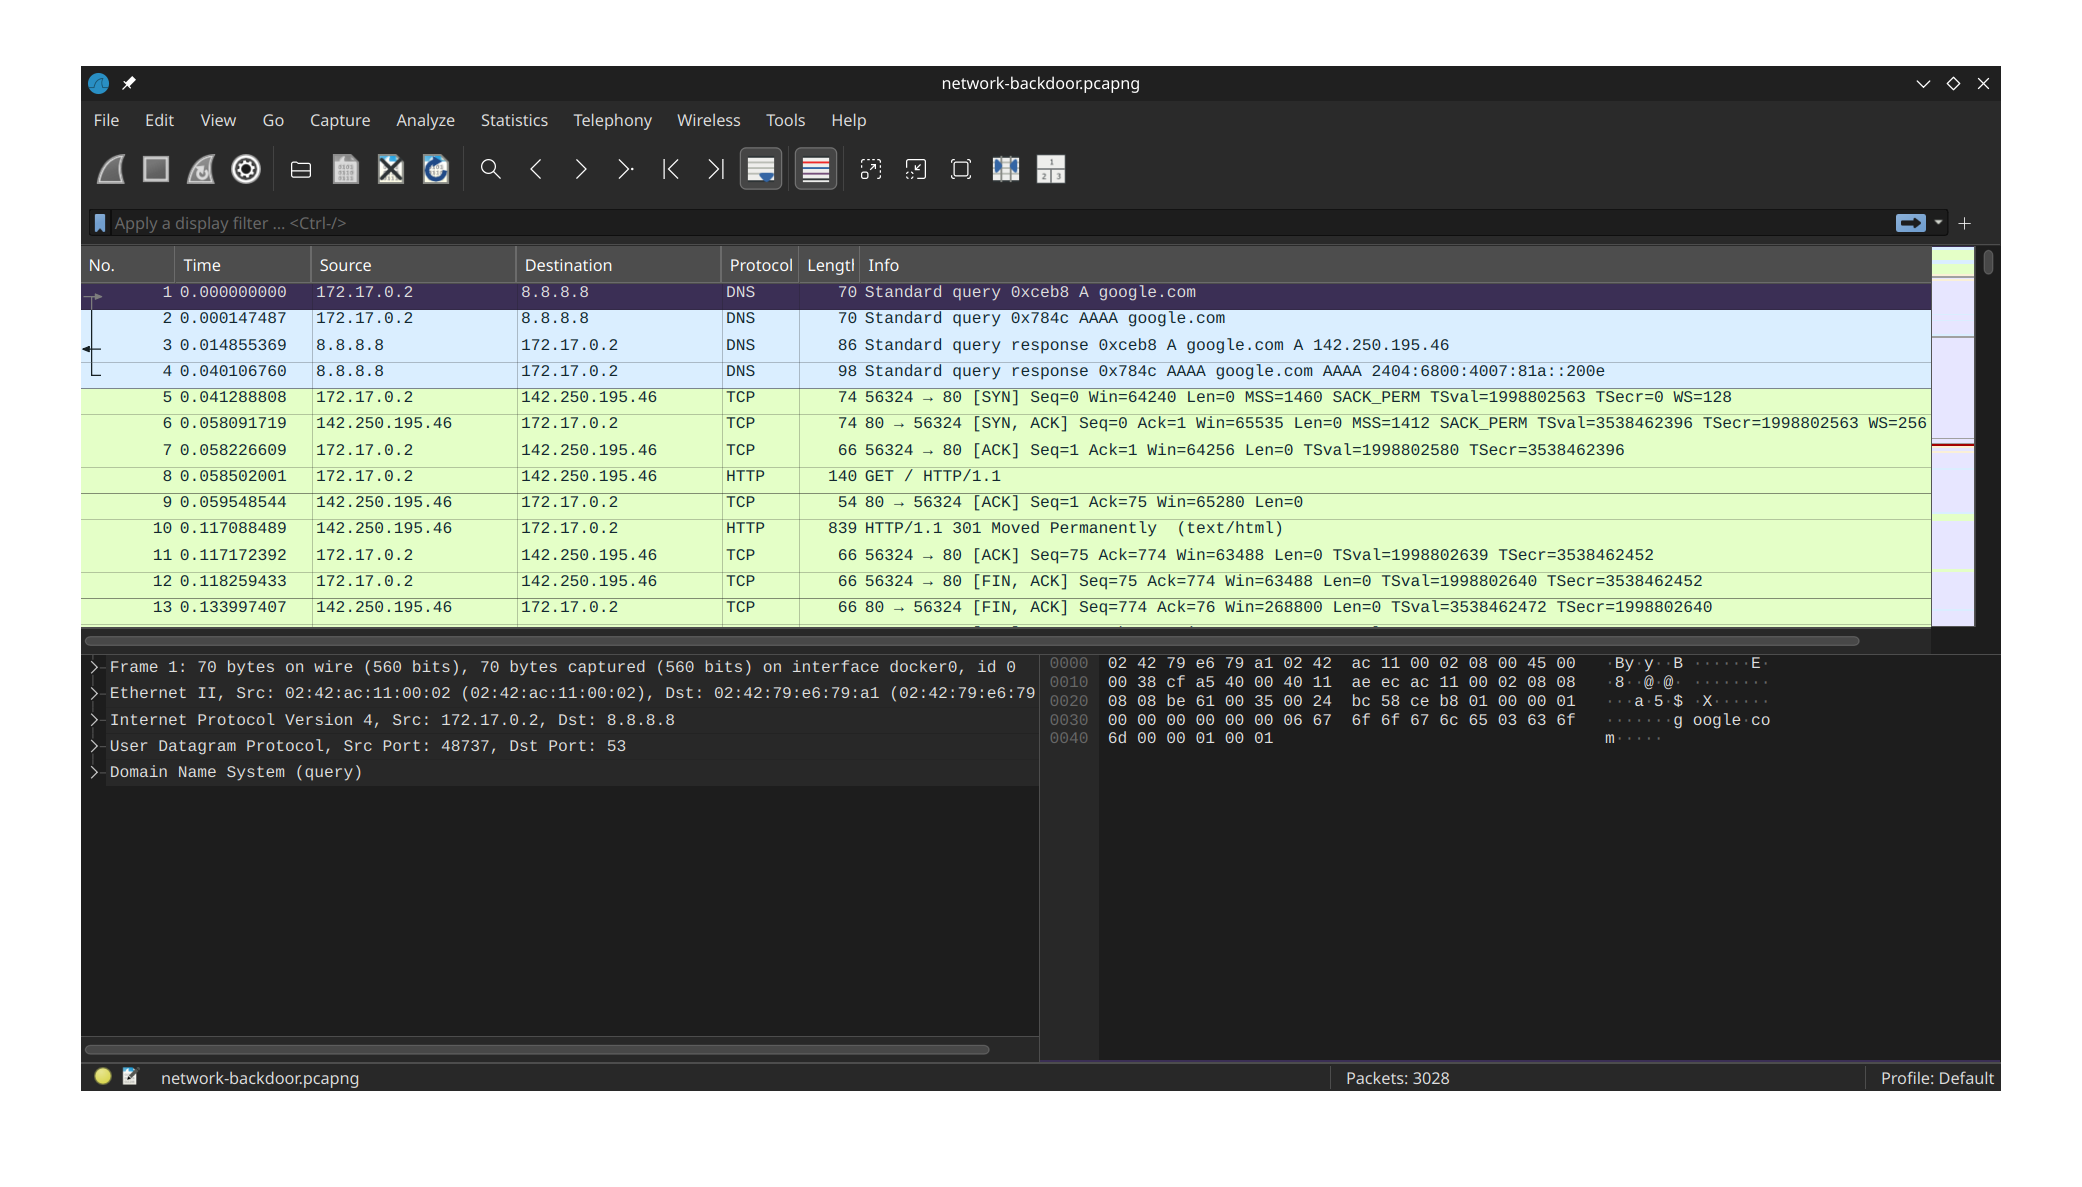
\includegraphics[width=0.8\textwidth]{1}
    \caption{Wireshark main interface showing captured packets}
\end{figure}

\subsection{Identifying Suspicious Traffic}
Inspect the packets for suspicious HTTP requests or command-and-control traffic. Pay particular attention to packets containing shell commands or command outputs.

\begin{figure}[H]
    \centering
    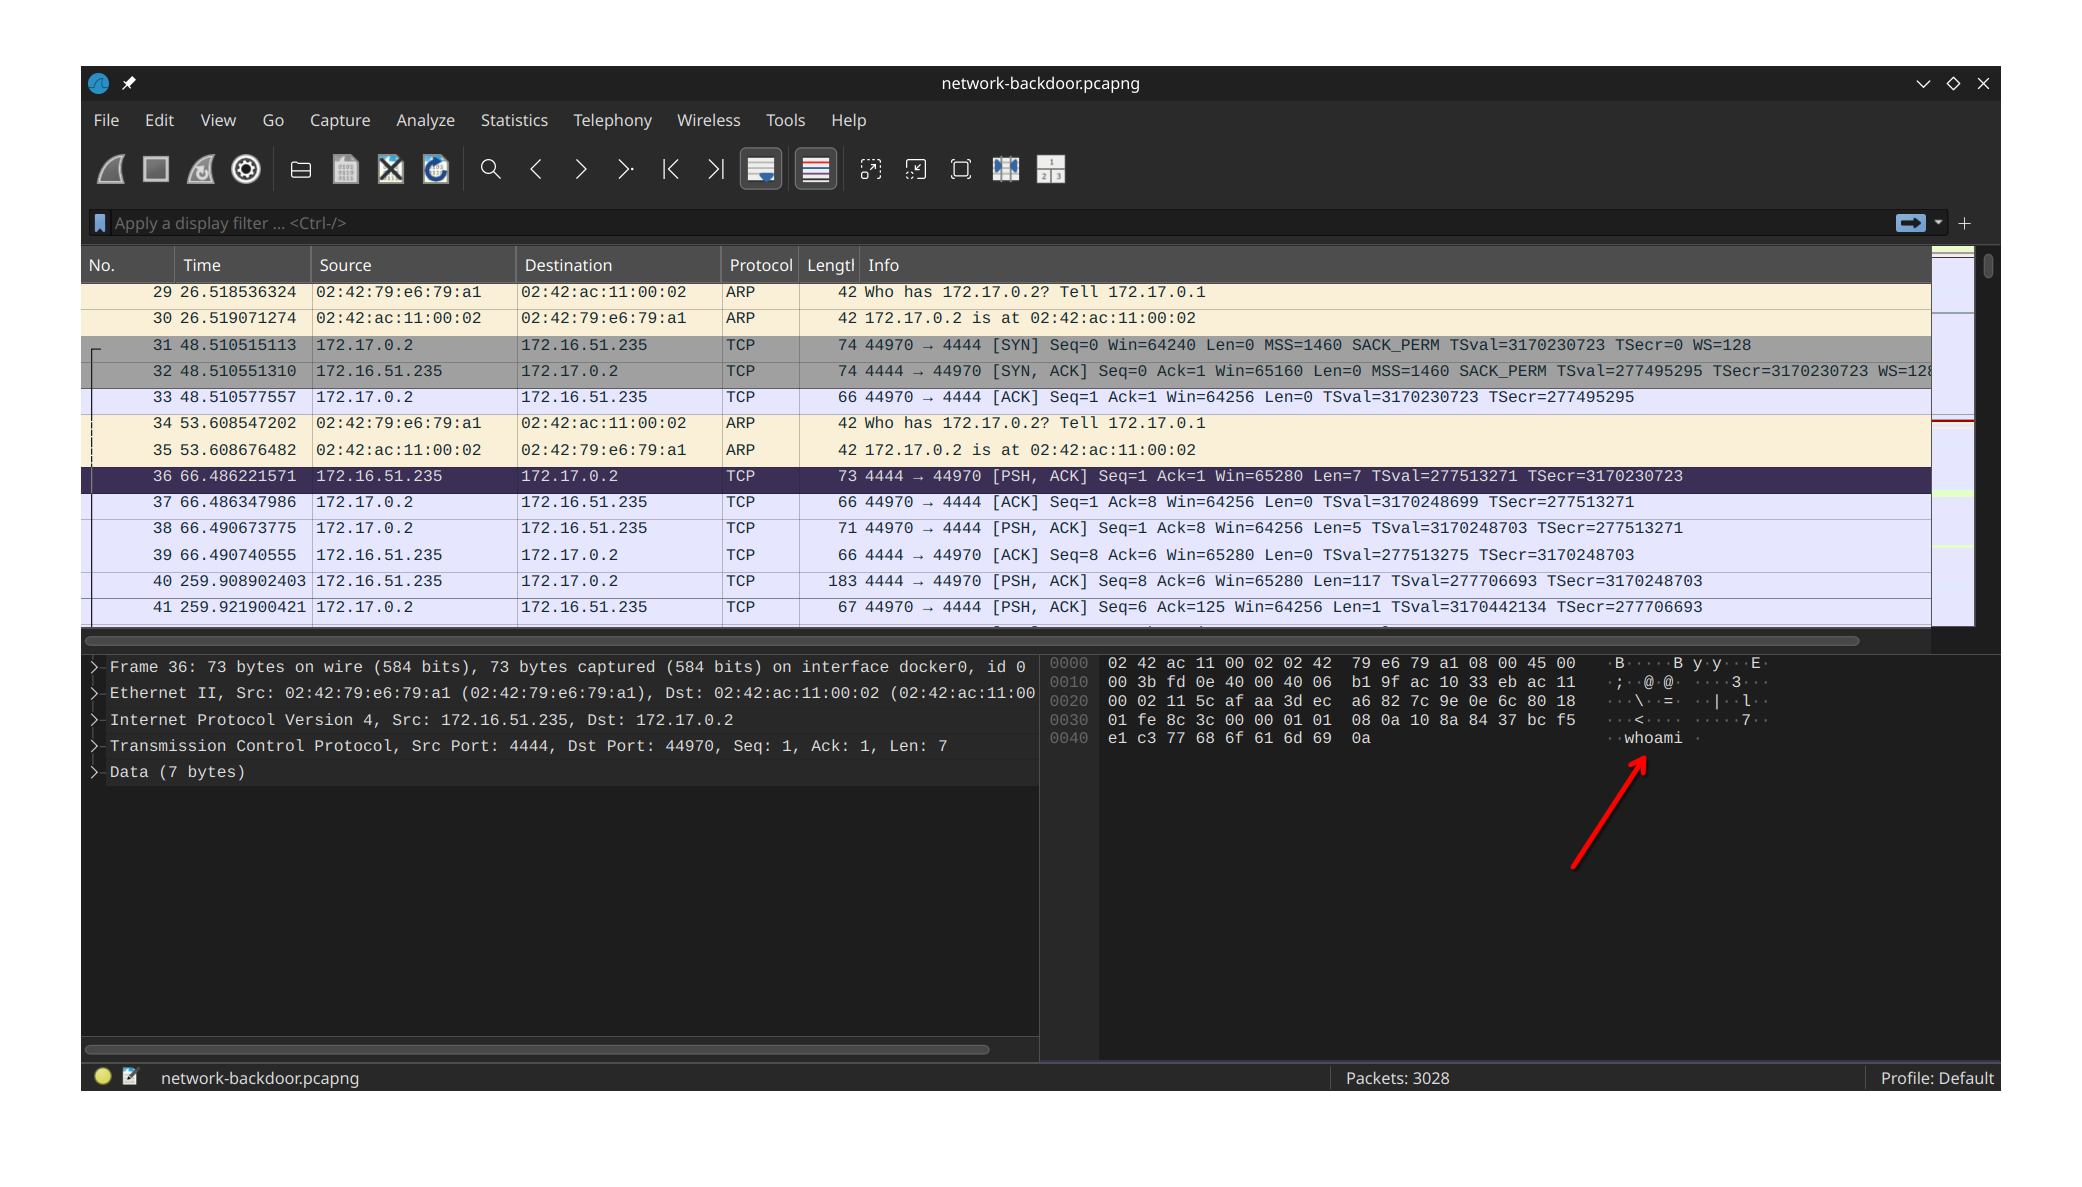
\includegraphics[width=0.8\textwidth]{2}
    \caption{Suspicious command traffic identified in packet capture}
\end{figure}

\subsection{TCP Stream Analysis}
To analyze the complete communication:
\begin{enumerate}
    \item Locate the first packet containing command traffic
    \item Right-click and select "Follow TCP Stream"
\end{enumerate}

\begin{figure}[H]
    \centering
    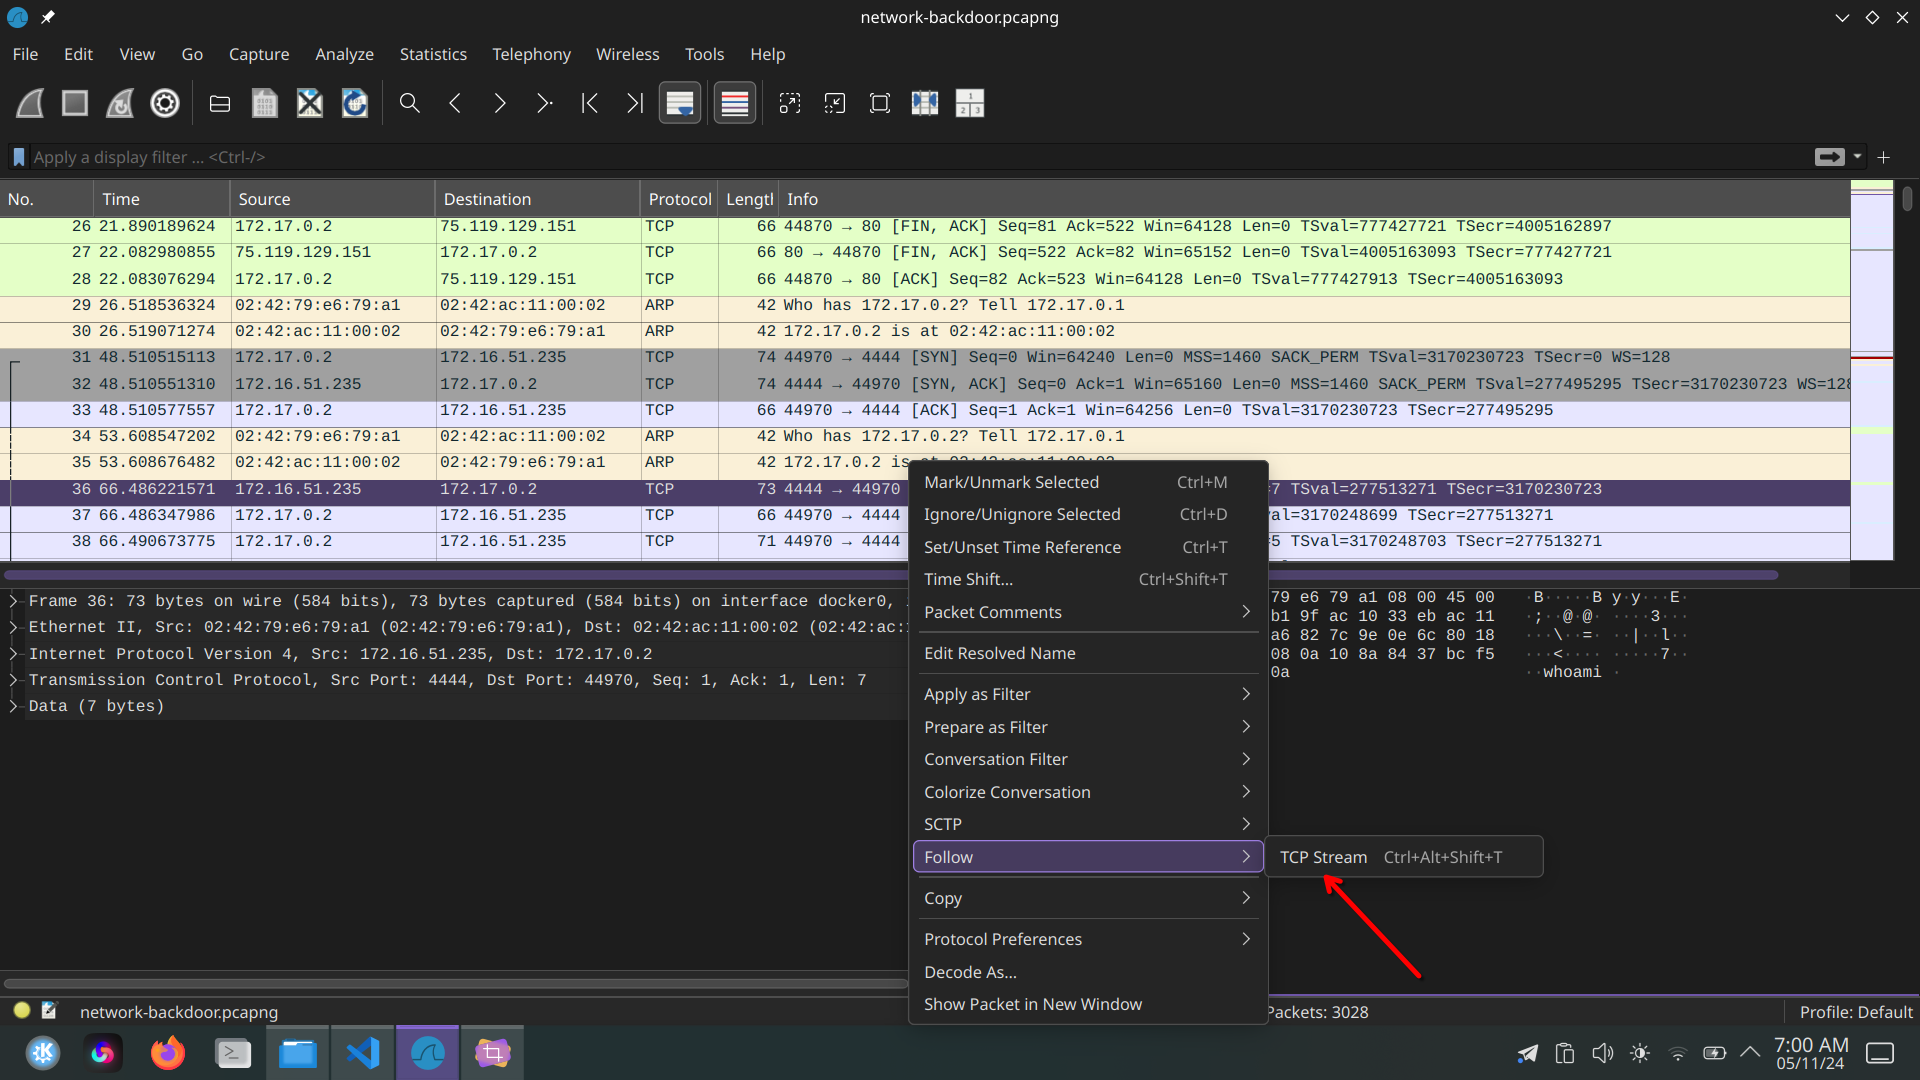
\includegraphics[width=0.8\textwidth]{3}
    \caption{TCP stream analysis showing command and control traffic}
\end{figure}

\subsection{Findings}
The analysis reveals:
\begin{itemize}
    \item Presence of backdoor communication
    \item Evidence of attempted trojan installation
\end{itemize}

\begin{figure}[H]
    \centering
    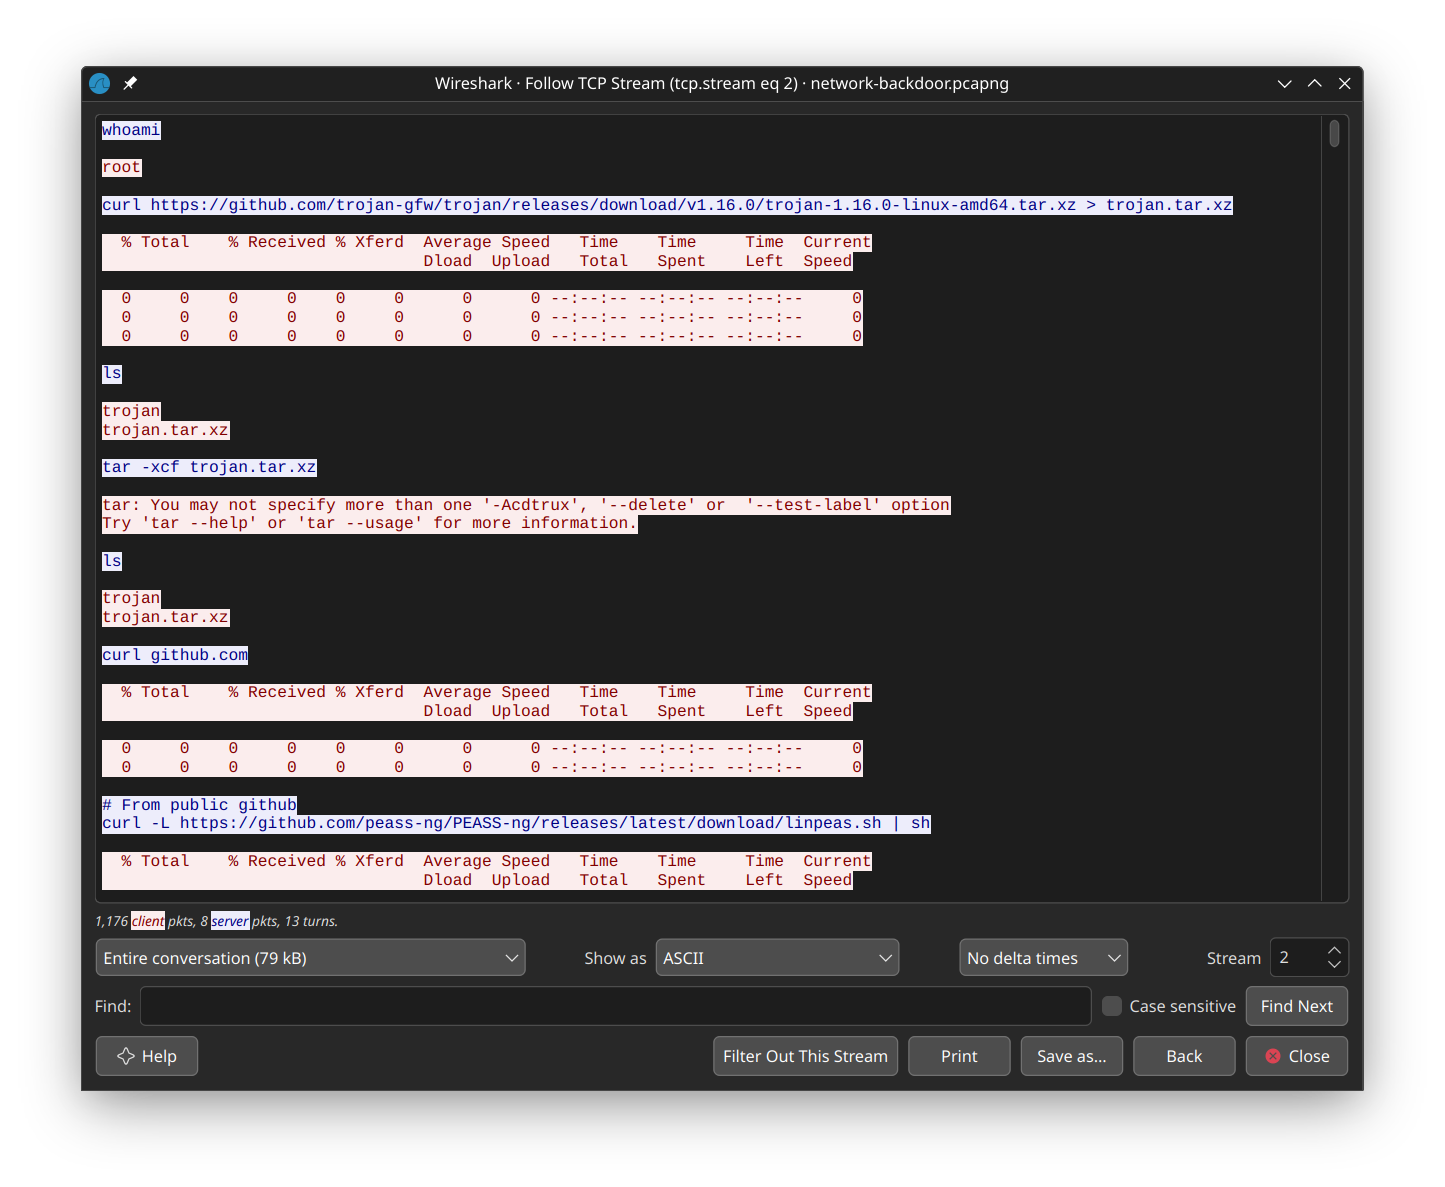
\includegraphics[width=0.8\textwidth]{4}
    \caption{Evidence of trojan installation attempt in network traffic}
\end{figure}

\end{document}
